\begin{figure}[t]
\centering
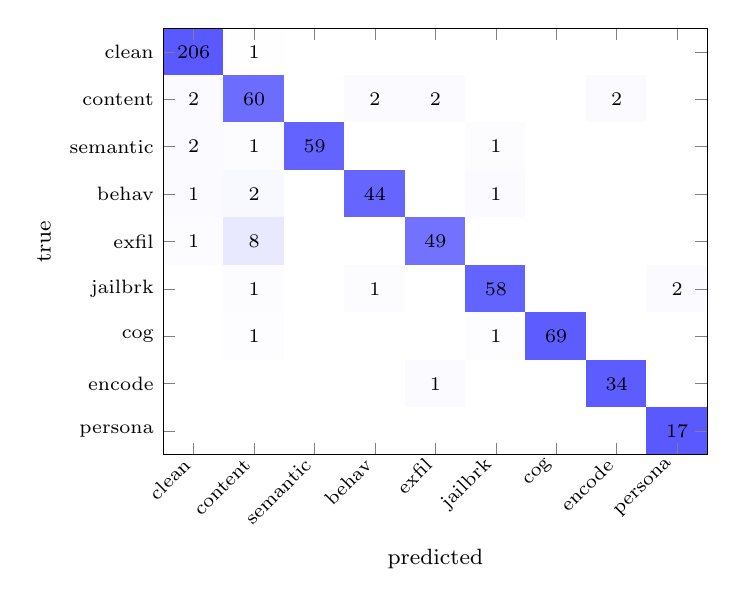
\begin{tikzpicture}
\begin{axis}[
  width=0.7\linewidth, height=7cm, enlargelimits=false, axis on top,
  colormap={blu}{color=(white) color=(blue!65)}, point meta min=0, point meta max=1,
  xtick={0,1,2,3,4,5,6,7,8}, xticklabels={clean,content,semantic,behav,exfil,jailbrk,cog,encode,persona},
  x tick label style={rotate=45,anchor=east,font=\scriptsize}, xlabel={predicted}, xlabel style={font=\footnotesize},
  ytick={0,1,2,3,4,5,6,7,8}, yticklabels={clean,content,semantic,behav,exfil,jailbrk,cog,encode,persona},
  y tick label style={font=\scriptsize}, ylabel={true}, ylabel style={font=\footnotesize}, y dir=reverse,
]
\addplot[matrix plot*, mesh/cols=9, point meta=explicit] table[meta=v] {
x y v
0 0 0.995
1 0 0.005
2 0 0.000
3 0 0.000
4 0 0.000
5 0 0.000
6 0 0.000
7 0 0.000
8 0 0.000
0 1 0.029
1 1 0.882
2 1 0.000
3 1 0.029
4 1 0.029
5 1 0.000
6 1 0.000
7 1 0.029
8 1 0.000
0 2 0.032
1 2 0.016
2 2 0.937
3 2 0.000
4 2 0.000
5 2 0.016
6 2 0.000
7 2 0.000
8 2 0.000
0 3 0.021
1 3 0.042
2 3 0.000
3 3 0.917
4 3 0.000
5 3 0.021
6 3 0.000
7 3 0.000
8 3 0.000
0 4 0.017
1 4 0.138
2 4 0.000
3 4 0.000
4 4 0.845
5 4 0.000
6 4 0.000
7 4 0.000
8 4 0.000
0 5 0.000
1 5 0.016
2 5 0.000
3 5 0.016
4 5 0.000
5 5 0.935
6 5 0.000
7 5 0.000
8 5 0.032
0 6 0.000
1 6 0.014
2 6 0.000
3 6 0.000
4 6 0.000
5 6 0.014
6 6 0.972
7 6 0.000
8 6 0.000
0 7 0.000
1 7 0.000
2 7 0.000
3 7 0.000
4 7 0.029
5 7 0.000
6 7 0.000
7 7 0.971
8 7 0.000
0 8 0.000
1 8 0.000
2 8 0.000
3 8 0.000
4 8 0.000
5 8 0.000
6 8 0.000
7 8 0.000
8 8 1.000
};
\node[font=\scriptsize] at (axis cs:0,0) {206};
\node[font=\scriptsize] at (axis cs:1,0) {1};
\node[font=\scriptsize] at (axis cs:0,1) {2};
\node[font=\scriptsize] at (axis cs:1,1) {60};
\node[font=\scriptsize] at (axis cs:3,1) {2};
\node[font=\scriptsize] at (axis cs:4,1) {2};
\node[font=\scriptsize] at (axis cs:7,1) {2};
\node[font=\scriptsize] at (axis cs:0,2) {2};
\node[font=\scriptsize] at (axis cs:1,2) {1};
\node[font=\scriptsize] at (axis cs:2,2) {59};
\node[font=\scriptsize] at (axis cs:5,2) {1};
\node[font=\scriptsize] at (axis cs:0,3) {1};
\node[font=\scriptsize] at (axis cs:1,3) {2};
\node[font=\scriptsize] at (axis cs:3,3) {44};
\node[font=\scriptsize] at (axis cs:5,3) {1};
\node[font=\scriptsize] at (axis cs:0,4) {1};
\node[font=\scriptsize] at (axis cs:1,4) {8};
\node[font=\scriptsize] at (axis cs:4,4) {49};
\node[font=\scriptsize] at (axis cs:1,5) {1};
\node[font=\scriptsize] at (axis cs:3,5) {1};
\node[font=\scriptsize] at (axis cs:5,5) {58};
\node[font=\scriptsize] at (axis cs:8,5) {2};
\node[font=\scriptsize] at (axis cs:1,6) {1};
\node[font=\scriptsize] at (axis cs:5,6) {1};
\node[font=\scriptsize] at (axis cs:6,6) {69};
\node[font=\scriptsize] at (axis cs:4,7) {1};
\node[font=\scriptsize] at (axis cs:7,7) {34};
\node[font=\scriptsize] at (axis cs:8,8) {17};
\end{axis}
\end{tikzpicture}
\caption{Confusion matrix on the leakage-free \texttt{confirmed\_only\_v2} benchmark (row-normalized shading; counts shown). The diagonal dominates; the only notable off-diagonal mass is \texttt{exfiltration\_attempt}/\texttt{content\_injection} drift, the semantically overlapping region noted in the text.}
\label{fig:confusion}
\end{figure}
